%************************************************
\section{Architettura del sistema di calcolo distribuito}
\label{sec:architettura}
%************************************************

\subsection{MPI}
\label{subsec:mpi}

MPI, acronimo per \emph{Message Passing Interface}, è un'interfaccia che permette lo scambio di dati tramite il paradigma di scambio di messaggi fra processi. 
Lo scambio può avvenire sia fra processi sulla stessa macchina (tipicamente tramite memoria condivisa), che fra processi su macchine differenti (tramite qualche protocollo di rete come TCP/IP).
Il principale vantaggio è l'indipendenza del codice dalla configurazione utilizzata. In altre parole, il programmatore che utilizza questa interfaccia non ha bisogno di sapere quanti processori avrà a disposizione e su quante macchine essi siano distribuiti, si dovrà semplicemente occupare di scambiare i dati con le primitive offerte dall'interfaccia, e il mezzo di comunicazione verrà poi determinato automaticamente a seconda dell'implementazione di MPI e della disponibilità di risorse.

\begin{figure}[p]
\centering
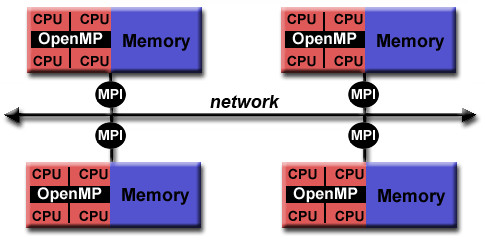
\includegraphics[scale=0.10]{hybrid_model.jpg}
\caption{Architettura ibrida}
\end{figure}
